\chapter{The quantum obstruction to local symmetry}
\label{chap:quantum-current-anomaly}

A holomorphic symmetry preserves the equations of the free
$\beta\gamma$ theory. Quantization must also preserve relations
between its current insertions. Contractions can violate those
relations when insertion points collide. The question is whether
a local failure remains when the heat cutoff tends to zero.

On $\mathbb C^2$, the first scalar failure comes from a triangle.
Two propagators and one heat kernel fill its four relative
antiholomorphic directions. A Gaussian integral then forces two
holomorphic derivatives onto the background fields. Its finite
limit is a local cubic functional. The coefficient depends on
the orientation, the odd pairing, and the normalization of the
connected expansion, which must be used together.

\section{Local symmetries and their sources}

Use the coordinates and orientation of
Chapter~\ref{chap:two-dimensional-free-fields}:
\[
 z_j=x_j+iy_j,\qquad \Omega=dz_1\wedge dz_2,\qquad
 dV_4=dx_1\wedge dy_1\wedge dx_2\wedge dy_2.
\]
Write the second full matter field as
$\beta_{\mathrm{full}}=\beta\wedge\Omega$.
Throughout this chapter, $\beta$ denotes this coefficient field.
The even holomorphic degree of $\Omega$ permits moving it to
the right without a sign. This fixes the volume convention
before any current or action formula.

Let $\mathfrak g$ be an ordinary finite-dimensional complex Lie
algebra, and let $\rho:\mathfrak g\to\operatorname{End}_{\mathbb C}(V)$
be a representation on an ordinary finite-dimensional complex
vector space. A smooth $\mathfrak g$-valued function $\varepsilon$
acts on the ordinary fields by
\[
 \delta_\varepsilon\gamma=\rho(\varepsilon)\gamma,
 \qquad
 \delta_\varepsilon\beta=-\beta\rho(\varepsilon).
\]
In the free action, their variations cancel except for
$\int\beta\rho(\bar\partial\varepsilon)\gamma\wedge\Omega$.
Thus holomorphic parameters act as symmetries. A general smooth
parameter exposes the local current coupled to
$\bar\partial\varepsilon$.

The differential graded Lie algebra of parameters is
\[
 \mathfrak g_c=\Omega_c^{0,\bullet}(\mathbb C^2,\mathfrak g),
 \qquad d=\bar\partial,
 \qquad
 [\alpha X,\eta Y]=(\alpha\wedge\eta)[X,Y].
\]
The subscript $c$ means compact support. The degree is the
antiholomorphic form degree. The topology on this space is the
usual inductive limit of smooth forms supported in fixed compact
sets, with uniform seminorms on every derivative.

To include relations between parameters, replace a single source
by a universal background $A$. Its component of form degree $q$
has ghost number $1-q$. Concretely, every formula can be evaluated
on a finite sum
\[
 A=\sum_a t_a\alpha_a,\qquad
 \alpha_a\in\mathfrak g_c^{p_a},\quad |t_a|=1-p_a,
\]
in a free graded commutative parameter algebra. An odd parameter
squares to zero. Even parameters are formal. Identities mean
identities of coefficients for every such finite family.
This defines the local polynomial functionals without choosing
a basis in an infinite-dimensional dual.

The matter fields are
\[
 \gamma\in\Omega^{0,\bullet}(\mathbb C^2,V),\qquad
 \beta\in\Omega^{0,\bullet}(\mathbb C^2)\otimes V^\vee[1].
\]
The shift convention is $E[k]^j=E^{j+k}$.
Here the shift acts on the coefficient space of $\beta$.
The component coordinates of $\gamma,\beta,A$ have ghost numbers
$-q,1-q,1-q$, respectively. Their total degrees, meaning ghost
number plus antiholomorphic form degree, are $0,1,1$.

Put ghost coefficients before forms. For homogeneous coefficients
$u,v$ and forms $\alpha,\eta$, use
\begin{equation}\label{eq:qca-totalization}
 (u\alpha)(v\eta)=(-1)^{|\alpha|\operatorname{gh}(v)}
                  uv\,\alpha\wedge\eta.
\end{equation}
The totalized spatial differential has the sign
$d(u\alpha)=(-1)^{\operatorname{gh}(u)}u\,d\alpha$
when $u$ is a formal coefficient. For coordinate-dependent
coefficients, the same rule applies to their spatial derivatives.
Write $d_{\mathrm{raw}}$ for ordinary coefficientwise Dolbeault
differentiation before this sign is inserted.
Holomorphic coordinate derivatives $\partial_i=\partial_{z_i}$
have degree zero. Every coordinate formula places $\Omega$ on
the right.

The graded-dual free differential on observables is denoted by
$Q$. On a linear coordinate $\phi$ it is
$(Q\phi)(e)=-(-1)^{|\phi|}\phi(de)$.
For components of form degree $q$, this gives
\[
 Q\gamma_q=(-1)^{q+1}d_{\mathrm{raw}}\gamma_{q-1},\qquad
 Q\beta_q=(-1)^q d_{\mathrm{raw}}\beta_{q-1}.
\]
Components with a negative index are zero. In the totalized
notation these equations read $Q\gamma=d\gamma$ and $Q\beta=d\beta$.

The Chevalley--Eilenberg differential on the background is
\begin{equation}\label{eq:qca-ce}
 d_{\mathrm{CE}}A=dA-A^2,
 \qquad d_{\mathrm{CE}}=d_{{\mathrm{CE}},1}+d_{{\mathrm{CE}},2}.
\end{equation}
The subscripts denote the linear and quadratic terms in $A$.
Its linear component is
$d_{{\mathrm{CE}},1}A_q=(-1)^q d_{\mathrm{raw}}A_{q-1}$.
The sign comes from the shifted dual
$\mathfrak g_c^\vee[-1]$. Both $d_{\mathrm{CE}}$ and $Q$ are left
derivations of ghost degree one. They anticommute with $d$ and
commute with $\partial_i$.
For example,
\[
 \begin{split}
 d_{\mathrm{CE}}^2A
 &=-d(dA-A^2)-(dA-A^2)A+A(dA-A^2)\\
 &=d(A^2)-(dA)A+A(dA)=0.
 \end{split}
\]
Here $d(A^2)=(dA)A-A(dA)$ because $A$ is odd.

Replace $A$ by $\rho(A)$ in matrix products, leaving the symbol
$A$ unchanged. The source interaction is
\begin{equation}
 I(A)=\int_{\mathbb C^2}\beta A\gamma\wedge\Omega.
\end{equation}
The integral selects antiholomorphic degree two, so $I$ has ghost
number zero. Compact support of $A$ makes it a functional on
arbitrary smooth matter fields. It is the generating function
for local current insertions, including their ghost components.

\section{Which contractions are defined}

A local current has a distribution kernel on the diagonal.
It therefore requires an observable space containing such kernels.
Let $E$ denote the finite-rank graded bundle of matter components.
Define
\[
 \mathcal O_{\mathrm{dist}}
 =\bigoplus_{n\geq0}
 \mathcal E'_c\bigl((\mathbb C^2)^n;
       (E^\vee)^{\boxtimes n}\otimes\operatorname{Dens}\bigr)_{S_n}.
\]
Here $\mathcal E'_c$ means compactly supported distribution
kernels, interpreted by pairing against smooth sections.
The subscript takes graded symmetric coinvariants.
The term $n=0$ is $\mathbb C$.
On each scalar component, such a kernel is a linear functional
$T$ on smooth tests for which some compact set $K$, integer
$m\geq0$, and constant $C$ satisfy
\[
 |T(\phi)|\leq C\max_{|\nu|\leq m}\sup_K|\partial^\nu\phi|.
\]
Here $\nu$ is a tuple of nonnegative integers, $|\nu|$ is its
sum, and derivatives use the real coordinates of the insertion
points. This estimate defines finite order and implies support
in $K$: the functional vanishes on tests zero near $K$.
A family of smooth tests is bounded if every derivative is
uniformly bounded on each fixed compact set.
The strong distribution topology is defined by the seminorms
$T\mapsto\sup_{\phi\in B}|T(\phi)|$ for these bounded families $B$.
Each seminorm is finite by the displayed estimate.

Products first keep the position variables separate. For scalar
kernels $T,S$, define
\[
 (T\boxtimes S)(\phi)
       =T\bigl(x\mapsto S(y\mapsto\phi(x,y))\bigr).
\]
Difference quotients of $\phi$ converge uniformly with all
derivatives needed by $S$ on its compact support.
Thus the inner function is smooth and its derivatives pass
through $S$. The two finite-order estimates give
\[
 |(T\boxtimes S)(\phi)|
 \leq C_TC_S
 \max_{\substack{|\mu|\leq m_T\\|\nu|\leq m_S}}
       \sup_{K_T\times K_S}|\partial_x^\mu\partial_y^\nu\phi|.
\]
This defines a compact distribution on the product.
It agrees with $T(f)S(g)$ on a separated test $f(x)g(y)$.
Finite sums of such tests approximate a smooth test with its
required derivatives on the compact product: multiply by
coordinate cutoffs and expand on a larger periodic box.
Repeated integration by parts makes its Fourier coefficients
decay faster than any prescribed power, so the differentiated
partial sums converge uniformly.
The estimate therefore determines the product uniquely from
separated tests. Interchanging or regrouping factors gives the
same product, with the graded sign for their coefficient labels.
Passing to graded symmetric coinvariants gives multiplication
on $\mathcal O_{\mathrm{dist}}$.
It involves no restriction of a product of distributions to a
diagonal.

The operator $Q$ differentiates these kernels by duality.
A smooth contraction kernel also acts: multiply a compact
distribution by its smooth coefficient and push forward along
the contracted coordinates. Compact support makes that pushforward
defined. This constructs all positive-scale operations used below.

The scalar kernels inherited from the free theory are
\begin{equation}
 \begin{split}
 N(u)&=\bar u_1d\bar u_2-\bar u_2d\bar u_1,\\
 p_t(u)&=\frac{e^{-|u|^2/(4t)}}{64\pi^2t^3}N(u),\\
 H_t(u)&=\frac{e^{-|u|^2/(4t)}}{64\pi^2t^2}
                     d\bar u_1\wedge d\bar u_2,\\
 P_{\epsilon,L}(u)&=\int_\epsilon^L p_t(u)\,dt,
                    \qquad 0<\epsilon<L<\infty.
 \end{split}
\end{equation}
All two-point forms use full differences, including
$d\bar u_j=d\bar z_j-d\bar w_j$ when $u=z-w$.
In particular, the pullback under $u\mapsto-u$ fixes both
$P_{\epsilon,L}$ and $H_t$.

These normalizations follow directly from the heat kernel
$k_t=(4\pi t)^{-2}e^{-|u|^2/(4t)}$ and the identity
$d\bar u_1\wedge d\bar u_2\wedge\Omega=4dV_4$.
Differentiation gives
\[
 dp_t=-\partial_tH_t,\qquad
 dP_{\epsilon,L}=H_\epsilon-H_L,
 \qquad H_t\wedge\Omega=k_t\,dV_4.
\]
As $\epsilon\to0$, the propagator tends coefficientwise away
from zero to
\[
 P_{0,L}(u)=\frac{N(u)}{4\pi^2|u|^4}
       \left(1+\frac{|u|^2}{4L}\right)e^{-|u|^2/(4L)}.
\]
Its coefficients are $O(|u|^{-3})$ near zero, hence locally
integrable in four real dimensions. Its differential is
$H_0-H_L$ as a current, where
$H_0\wedge\Omega=\delta_0dV_4$.

The odd pairing contracts a $\beta$ component with a $\gamma$
component by evaluation $V^\vee\otimes V\to\mathbb C$.
For a homogeneous symmetric kernel tensor
$M=\sum_j e_j\otimes f_j$, write
$\partial_M=\frac12\sum_j\partial_{e_j}\partial_{f_j}$,
using left derivatives for odd coordinates. Let $K_t$ be the
heat tensor induced by $H_t$ and this pairing. Set
\begin{equation}\label{eq:qca-operators}
 \Delta_t=-\partial_{K_t},\qquad
 \mathcal C_{\epsilon,L}=\partial_{P_{\epsilon,L}},\qquad
 [Q,\mathcal C_{\epsilon,L}]=\Delta_\epsilon-\Delta_L.
\end{equation}
The pairing is included in the last propagator notation.
The operators $Q,\Delta_t$ have degree one, and
$\mathcal C_{\epsilon,L}$ has degree zero.
These are the same tensor-to-operator signs as
\eqref{eq:gaussian-scale-operators}.

For distinct vertices $i,j$, the contraction reads
\[
 \mathcal C_{ij}=P_{\epsilon,L}(z_i-z_j)
 \sum_a\left(
   \partial_{\beta_a(i)}\partial_{\gamma_a(j)}
  +\partial_{\gamma_a(i)}\partial_{\beta_a(j)}\right).
\]
Its odd differential form is on the left. Replacing $P$ by $H_t$
gives the raw heat contraction. Its negative is the
Batalin--Vilkovisky (BV) operator.
For instance, the commutator on a paired bilinear has kernel
$-dP=-(H_\epsilon-H_L)$, which proves the sign in
\eqref{eq:qca-operators} on a paired bilinear.

General joint kernels require the same identity on all their
smooth tests. Let $T$ be an $n$-slot distribution kernel, and
let $\pi_{ij}$ forget slots $i,j$. A smooth test $\psi$ in the
remaining slots gives the contraction
\[
 (\mathcal C_{ij}T)(\psi)
       =T\bigl[P_{ij}\,\pi_{ij}^*\psi\bigr].
\]
In this formula $P_{ij}$ includes the pairing bivector in the
selected slots. Insert it into the full ordered list of slots
using the graded permutation rule. This specifies the signs
and the test section, including its coefficient labels.
The kernel $P_{\epsilon,L}$ is smooth, so the test is smooth.
Compact support of $T$ makes the resulting distribution compact.

Transpose $Q$ onto this test and use the product rule.
The terms differentiating $\psi$ cancel between
$Q\mathcal C_{ij}$ and $\mathcal C_{ij}Q$.
The remaining term inserts $-dP_{ij}$, with the bilinear sign
computed above. Since $-dP_{ij}=-H_{\epsilon,ij}+H_{L,ij}$,
summing over all pairs proves
\eqref{eq:qca-operators} on every joint distribution kernel.
This argument does not require a decomposition into products
of linear measurement kernels.

The BV bracket at scale $t>0$ is
\[
 \{F,G\}_t=(-1)^{|F|}
 \bigl(\Delta_t(FG)-(\Delta_tF)G
                    -(-1)^{|F|}F\Delta_tG\bigr).
\]
It has degree one and obeys
$\{F,G\}_t=-(-1)^{(|F|+1)(|G|+1)}\{G,F\}_t$.
Two successive contractions choose disjoint pairs of slots.
Exchanging their order reverses the sign because each heat
contraction has degree one. Their terms cancel, proving
$\Delta_t^2=0$ on arbitrary joint kernels.
The preceding transposed-test argument and $dH_t=0$ give
$Q\Delta_t+\Delta_tQ=0$ on that same space.
In the bracket, contractions within either factor cancel;
only pairs joining the two factors remain.
Each term in its Jacobi identity therefore chooses two
pairings connecting three input groups.
The same pairings occur in two orders among the nested
brackets. The graded permutation signs and the odd degree of
each contraction make their coefficients opposite.
Their pairwise cancellation proves the graded Jacobi identity.
The notation $\{-,-\}_0$ below refers only to the explicit
local brackets for which the diagonal evaluation exists.

The locally integrable $P_{0,L}$ defines the particular tree
kernels below. It does not define an operator on all of
$\mathcal O_{\mathrm{dist}}$: multiplication of an arbitrary
distribution by this singular coefficient has no general meaning.
Every use of a singular propagator will therefore have its own
integrability argument.

\section{The classical identity and the first two currents}

The classical master identity expresses equivariance of the
source interaction. It also fixes its sign relative to the
contractions. Since $\beta$ and $A$ are odd,
\[
 QI=\int\bigl((d\beta)A\gamma+\beta A\,d\gamma\bigr)\wedge\Omega
    =\int\beta(dA)\gamma\wedge\Omega.
\]
The second equality integrates $d(\beta A\gamma)$ and uses
compact support. Equation~\eqref{eq:qca-ce} gives
\[
 d_{\mathrm{CE}}I=-\int\beta(dA-A^2)\gamma\wedge\Omega.
\]
One diagonal contraction between two copies of $I$ gives
\[
 \frac12\{I,I\}_0=-\int\beta A^2\gamma\wedge\Omega.
\]
The two possible contractions cancel the factor $1/2$.
Their minus sign is the heat sign in
\eqref{eq:qca-operators}, with the odd coordinate derivatives
acting from the left. Thus
\begin{equation}\label{eq:qca-cme}
 (Q+d_{\mathrm{CE}})I+\frac12\{I,I\}_0=0.
\end{equation}
This is the classical master equation for the local symmetry.

At a positive scale, its binary bracket is spread over the heat
kernel. A bilocal current compensates for that change. Put
\[
 I_1(A)=I(A),\qquad
 I_2^{\epsilon,L}(A)=
       \frac12\mathcal C_{\epsilon,L}(I(A)^2)_{\mathrm{connected}}.
\]
The subscript retains contractions joining the two vertices.
One-edge differentiation gives the explicit positive expression
\begin{equation}
 I_2^{0,L}(A)=\int_{(\mathbb C^2)^2}
 P_{0,L}(z-w)\,
 \beta(z)A(z)A(w)\gamma(w)\wedge\Omega_z\wedge\Omega_w.
\end{equation}
The factor $1/2$ cancels the two orders of the vertices.
The kernel is compactly supported in the background variables,
and $P_{0,L}$ is locally integrable in $z-w$.
Thus it defines a quadratic observable distribution kernel.

Let $d_0=Q+d_{{\mathrm{CE}},1}$. The linear part of
\eqref{eq:qca-cme} gives $d_0I_1=0$.
Using \eqref{eq:qca-operators} on $I_1^2$ gives
\[
 d_0I_2^{\epsilon,L}
 =\frac12\bigl(\{I_1,I_1\}_\epsilon-\{I_1,I_1\}_L\bigr).
\]
Since $d_{{\mathrm{CE}},2}I_1=-\frac12\{I_1,I_1\}_0$,
\[
 d_0I_2^{\epsilon,L}+d_{{\mathrm{CE}},2}I_1
       +\frac12\{I_1,I_1\}_L
 =\frac12\bigl(\{I_1,I_1\}_\epsilon-\{I_1,I_1\}_0\bigr).
\]
The heat kernel is an approximate identity on smooth compact
coefficients. Its right side tends to zero as a distribution.
Consequently the first two Ward identities are
\begin{equation}
 d_0I_1=0,\qquad
 d_0I_2^{0,L}+d_{{\mathrm{CE}},2}I_1
                   +\frac12\{I_1,I_1\}_L=0.
\end{equation}

For the corresponding graded maps, let
$\mathcal L_L=\mathcal O_{\mathrm{dist}}[[\hbar]][-1]$.
Write $uF$ for a shifted observable, so $|uF|=|F|+1$, and put
\[
 d_{\mathcal L_L}(uF)=-u(Q+\hbar\Delta_L)F,
 \qquad [uF,uG]_L=u\{F,G\}_L.
\]
This is a differential graded Lie algebra.
For $\alpha\in\mathfrak g_c^p$ and $\eta\in\mathfrak g_c^q$, define
\[
 \begin{split}
 J(\alpha)&=\int\beta\rho(\alpha)\gamma\wedge\Omega,\\
 K_L(\alpha,\eta)&=\int P_{0,L}(z-w)\,
       \beta(z)\rho(\alpha(z))\rho(\eta(w))\gamma(w)
                    \wedge\Omega_z\wedge\Omega_w.
 \end{split}
\]
Their ghost degrees are $p-1$ and $p+q-2$.
The actual first and second Noether components are
\begin{equation}\label{eq:qca-noether-components}
 \begin{split}
 F_1(\alpha)&=(-1)^{p+1}uJ(\alpha),\\
 F_2(\alpha,\eta)&=(-1)^{p+q+1}u
       \bigl(K_L(\alpha,\eta)-(-1)^{pq}K_L(\eta,\alpha)\bigr).
 \end{split}
\end{equation}
They have degrees $0,-1$. The second is graded antisymmetric.

\begin{proposition}\label{prop:qca-noether-two}
The maps in \eqref{eq:qca-noether-components} satisfy
\[
 \begin{split}
 d_{\mathcal L_L}F_1(\alpha)&=F_1(d\alpha),\\
 d_{\mathcal L_L}F_2(\alpha,\eta)
   +F_2(d\alpha,\eta)+(-1)^pF_2(\alpha,d\eta)
 &=F_1([\alpha,\eta])-[F_1(\alpha),F_1(\eta)]_L.
 \end{split}
\]
\end{proposition}

\begin{proof}
Integration by parts gives $QJ(\alpha)=J(d\alpha)$.
Let $K_{H_t}$ denote the formula for $K_L$ with $P_{0,L}$
replaced by $H_t$. Differentiating that formula, including the
odd form $P$ on the left, gives
\[
 QK_L(\alpha,\eta)+K_L(d\alpha,\eta)
       +(-1)^pK_L(\alpha,d\eta)
 =-K_{H_0-H_L}(\alpha,\eta).
\]
The heat bracket has the direct contraction formula
\[
 \{J(\alpha),J(\eta)\}_L
 =-\bigl(K_{H_L}(\alpha,\eta)
               -(-1)^{pq}K_{H_L}(\eta,\alpha)\bigr).
\]
At $t=0$, the same difference is $J([\alpha,\eta])$.
Multiplying by the signs in
\eqref{eq:qca-noether-components} proves both identities with $Q$.

The additional $\Delta_L$ terms vanish.
For $J$, the full difference heat form pulls back to zero on
the diagonal. For $K_L$, its product with the propagator has
relative antiholomorphic degree three in two relative complex
coordinates, and is zero away from the diagonal. The product
is locally integrable, so it is the zero distribution.
Thus the identities hold with $Q+\hbar\Delta_L$.
\end{proof}

The second identity compares a pointwise parameter bracket with
a bilocal observable bracket. The explicit kernel supplies its
homotopy. Relations with three or more parameters require further
components and are not consequences of these two equations.

\section{Connected contractions and the quantum equation}

Introduce a formal variable $a$ which counts background order.
At positive cutoffs, use the algebra
\[
 \mathcal O_{\mathrm{dist}}[\hbar,\hbar^{-1}][[a]],
\]
with the graded parameter coefficients of $A$ included.
Each coefficient is a polynomial in matter fields and a finite
Laurent polynomial in $\hbar$. The lower Laurent bound can depend
on the power of $a$. Completion means coefficientwise agreement
below each fixed background order. Replace $I$ by $aI$ and define
\begin{equation}
 I_{\epsilon,L}
 =\hbar\log\left(e^{\hbar\mathcal C_{\epsilon,L}}
                         e^{aI/\hbar}\right).
\end{equation}
The formal logarithm is defined because its argument is $1+O(a)$.
At each background order, every contraction lowers matter degree
by two, so only finitely many contractions act.
The coefficient $a^n$ will be called background order $n$.
In this notation the background differential is
$d_{\mathrm{CE}}^{(a)}=d_{\mathrm{CE},1}+a\,d_{\mathrm{CE},2}$.
The extra $a$ records the increase of background order under
the quadratic term. This differential again squares to zero.

The logarithm retains connected graphs. This follows directly
from the exponential formula: a graph splits uniquely into
connected components, and the factorials in the exponential
count their unordered collections. Each vertex of $I$ has one
$\beta$ leg and one $\gamma$ leg. A connected graph is therefore
a path with two external matter legs or a closed directed cycle.
For $n$ vertices and $e$ contractions, its power of $\hbar$ is
$e-n+1$. Paths have power zero, and cycles have power one.

Write the terms through order three as
\[
 I_{\epsilon,L}
  =aI_1+a^2I_2^{\epsilon,L}
      +a^3\bigl(I_3^{\mathrm{tree}}[\epsilon,L]
                         +\hbar I_3^{\mathrm{loop}}[\epsilon,L]\bigr)
      +O(a^4).
\]
Here
\begin{equation}
 I_3^{\mathrm{tree}}=\frac1{12}\mathcal C_{\epsilon,L}^2(I^3)_{\mathrm{conn}},
 \qquad
 I_3^{\mathrm{loop}}=\frac1{36}\mathcal C_{\epsilon,L}^3(I^3)_{\mathrm{full}}.
\end{equation}
The factors are $1/(3!2!)$ and $1/(3!3!)$.
The subscripts retain connected trees and full contractions,
respectively. A one-vertex contraction vanishes because $P(0)=0$.
A two-vertex loop contains $P(z-w)^2=0$.
The latter equality uses the same scalar one-form on both edges,
including its full difference differential.

If the limits as $\epsilon\to0$ exist, denote them by $I_L$
through the indicated background order. Its failure to satisfy
the quantum master equation (QME) is
\begin{equation}\label{eq:qca-qme-defect}
 \mathcal R_L=(Q+d_{\mathrm{CE}}^{(a)})I_L
           +\frac12\{I_L,I_L\}_L+\hbar\Delta_LI_L.
\end{equation}
The QME asks for $\mathcal R_L=0$.
The term involving $\Delta_L$ accounts for a contraction inside
one observable. The bracket accounts for contractions between two
observables. This interpretation follows by applying
$Q+d_{\mathrm{CE}}^{(a)}+\hbar\Delta_L$ to $e^{I_L/\hbar}$ and dividing by
that exponential.

The scalar cubic component has only two terms:
\begin{equation}\label{eq:qca-scalar-component}
 [\mathcal R_L]_{\hbar,a^3,\mathrm{scalar}}
 =\hbar a^3\bigl(d_{{\mathrm{CE}},1}I_3^{\mathrm{loop}}[L]
                              +\Delta_LI_3^{\mathrm{tree}}[L]\bigr).
\end{equation}
Indeed, a bracket of two quadratic matter functionals remains
quadratic, and brackets with scalar functionals vanish.
The lower scalar loops are zero. The remaining contraction closes
a three-vertex path into a triangle with a marked heat edge.

\section{The marked triangle}

Put the marked edge between vertices $1$ and $2$, and write
\[
 x=z_1-z_3,\qquad y=z_2-z_3,\qquad z=z_3.
\]
The kernels, in their wedge order, are
$H_\epsilon(x-y)p_t(y)p_s(x)$.
Their geometry is the triangle
\[
 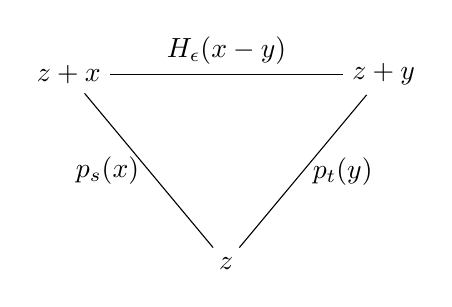
\begin{tikzpicture}[baseline=(current bounding box.center)]
  \node (one) at (-2,1) {$z+x$};
  \node (two) at (2,1) {$z+y$};
  \node (three) at (0,-1.4) {$z$};
  \draw (one) -- node[above] {$H_\epsilon(x-y)$} (two);
  \draw (two) -- node[right] {$p_t(y)$} (three);
  \draw (three) -- node[left] {$p_s(x)$} (one);
 \end{tikzpicture}
\]
The drawing records edges. Matter orientations will be counted
separately.

The relative antiholomorphic numerator is
\begin{equation}\label{eq:qca-exterior-numerator}
 \begin{split}
 &d(\bar x_1-\bar y_1)d(\bar x_2-\bar y_2)N(y)N(x)\\
 &\quad=(\bar x_2\bar y_1-\bar x_1\bar y_2)
                d\bar x_1d\bar x_2d\bar y_1d\bar y_2.
 \end{split}
\end{equation}
Products of differentials in this calculation mean wedge products.
To see the sign, the first two factors can contribute one $x$
and one $y$ differential in either order. The surviving terms
are $+\bar x_2\bar y_1$ and $-\bar x_1\bar y_2$ after ordering
the four differentials as displayed.

Set $T=\epsilon+s+t$. For each complex coordinate, the scalar
Gaussian has exponent $-\bar w^{\mathsf T}Mw$, where $w=(x_i,y_i)$
and
\[
 M=\frac14
 \begin{pmatrix}
  \epsilon^{-1}+s^{-1}&-\epsilon^{-1}\\
  -\epsilon^{-1}&\epsilon^{-1}+t^{-1}
 \end{pmatrix},\qquad
 \det M=\frac{T}{16\epsilon st}.
\]
Completing the square proves
$\int_{\mathbb C^2}e^{-\bar w^{\mathsf T}Mw}dV_w
=\pi^2/\det M$. Equivalently, diagonalize the positive real
symmetric matrix $M$ and use
$\int_{\mathbb C}e^{-\lambda|v|^2}dV_v=\pi/\lambda$.
Differentiation with respect to matrix entries, or integration
by parts, gives the normalized covariance $C=M^{-1}$:
\begin{equation}\label{eq:qca-covariance}
 C=\frac4T
 \begin{pmatrix}
  s(\epsilon+t)&st\\ st&t(\epsilon+s)
 \end{pmatrix},\qquad
 Z=(4\pi)^4\frac{\epsilon^2s^2t^2}{T^2}.
\end{equation}
The number $Z$ is the integral over all four complex relative
coordinates. The two coordinate pairs are independent.

For a normalized expectation $\mathbb E$, integration by parts
gives
\[
 \mathbb E[\bar w_a\Phi]
       =\sum_bC_{ba}\mathbb E[\partial_{w_b}\Phi].
\]
The boundary term vanishes for a smooth compact coefficient.
The identity also holds for polynomials because of Gaussian decay.
Apply it twice to the determinant in
\eqref{eq:qca-exterior-numerator}. The diagonal derivative terms
cancel, leaving
\begin{equation}
 \begin{split}
 &\mathbb E[(\bar x_2\bar y_1-\bar x_1\bar y_2)\Phi]\\
 &\qquad=-\frac{16\epsilon st}{T}
  \mathbb E[(\partial_{x_1}\partial_{y_2}
                  -\partial_{x_2}\partial_{y_1})\Phi].
 \end{split}
\end{equation}
The coefficient is $C_{xy}^2-C_{xx}C_{yy}=-\det C$.
For $\Phi=x_1y_2$, this is the deciding moment itself.

The relative holomorphic volume forms add a factor $16$,
because each relative identity is
$d\bar x_1d\bar x_2\Omega_x=4dV_x$.
Combining the three kernel denominators, $Z$, this factor,
and $-\det C$ gives
\[
 \frac{16Z}{(64\pi^2)^3\epsilon^2t^3s^3}
       \left(-\frac{16\epsilon st}{T}\right)
       =-\frac{\epsilon}{4\pi^2T^3}.
\]
This calculation includes every geometric normalization.

To express the resulting distribution, project the external
forms to the base $z$. Relative components vanish against the
relative top form in \eqref{eq:qca-exterior-numerator}.
Let $\Phi(z;x,y)$ denote the coefficient of the remaining base
$(0,2)$-form. With
$D_{xy}=\partial_{x_1}\partial_{y_2}-\partial_{x_2}\partial_{y_1}$,
the marked integral is exactly
\begin{equation}\label{eq:qca-marked-distribution}
 -\frac1{4\pi^2}\int_\epsilon^L\!\int_\epsilon^L
 \frac{\epsilon\,ds\,dt}{(\epsilon+s+t)^3}
 \int_{\mathbb C^2_z}\mathbb E[D_{xy}\Phi(z;x,y)]
                   \,d\bar z_1d\bar z_2\wedge\Omega_z.
\end{equation}
For products of compact backgrounds, $\Phi$ and all derivatives
have common compact support in these coordinates.

The mass in the time variables is elementary:
\begin{equation}\label{eq:qca-time-mass}
 \begin{split}
 \int_\epsilon^L\!\int_\epsilon^L
          \frac{\epsilon\,ds\,dt}{(\epsilon+s+t)^3}
 &=\frac16-\frac{\epsilon}{L+2\epsilon}
                    +\frac{\epsilon}{2(2L+\epsilon)}\\
 &=\frac{(L-\epsilon)^2}
                 {3(L+2\epsilon)(2L+\epsilon)}.
 \end{split}
\end{equation}
The first integration uses the antiderivative
$-\epsilon/[2(\epsilon+s+t)^2]$.
The second gives the three displayed fractions.
The limit at fixed $L>0$ is $1/6$.

\begin{lemma}\label{lem:qca-localization}
For smooth compact external coefficients, the marked triangle
converges as a distribution to
\[
 -\frac1{24\pi^2}\int_{\mathbb C^2_z}
        (D_{xy}\Phi)(z;0,0)
                     \,d\bar z_1d\bar z_2\wedge\Omega_z.
\]
At fixed $L$, the error is bounded by
$C_\Phi\sqrt\epsilon+C'_\Phi\epsilon/L$.
\end{lemma}

\begin{proof}
The covariance satisfies
$\mathbb E(|x|+|y|)\leq C\sqrt{s+t}$.
The mean-value theorem bounds the difference between
$\mathbb E[D_{xy}\Phi]$ and $(D_{xy}\Phi)(z;0,0)$ by
$C_\Phi\sqrt{s+t}$, with three derivatives of $\Phi$.
Its integrated contribution is bounded by
\[
 C_\Phi\int_\epsilon^L\!\int_\epsilon^L
       \frac{\epsilon\sqrt{s+t}}{(\epsilon+s+t)^3}\,ds\,dt
 \leq C'_\Phi\sqrt\epsilon.
\]
Indeed, set $s=\epsilon u,t=\epsilon v$.
The remaining integral on $u,v\geq1$ is bounded by a constant
times $\int_2^\infty r^{-3/2}dr$.
Equation~\eqref{eq:qca-time-mass} bounds the remaining error by
$C''_\Phi\epsilon/L$. These seminorm bounds prove distributional
convergence and support on the small diagonal.
\end{proof}

The other heat endpoint will occur in
\eqref{eq:qca-scalar-component}. Replacing $\epsilon$ by $L$ in
the heat edge and integrating the two propagator times over
$[0,L]$ gives
\[
 \int_0^L\!\int_0^L\frac{L\,ds\,dt}{(L+s+t)^3}=\frac16.
\]
Its covariance is bounded by $CL$. The same mean-value argument
gives localization with error $C_\Phi\sqrt L$ as $L\to0$.
Both endpoint descriptions therefore have marked geometric
coefficient $-1/(24\pi^2)$.

\section{Odd contractions and the trace coefficient}

The geometric integral must be multiplied by the coefficient
from Wick contractions. First take $V=\mathbb C$ and write
$I_i=\beta_iA_i\gamma_i$. Here $\beta_i,A_i$ are odd and
$\gamma_i$ is even. The propagator form is odd and stays on the
left of each contraction operator.

For one orientation with heat edge $12$, apply the propagator
derivatives on edges $13$ and $23$ first. With a fixed order of
the odd variables, the successive terms are
\[
 \begin{split}
 &P_{13}\partial_{\beta_1}\partial_{\gamma_3}
       (I_1I_2I_3)
       =-P_{13}\beta_2\beta_3A_1A_2A_3\gamma_1\gamma_2,\\
 &P_{23}\partial_{\beta_3}\partial_{\gamma_2}
       \bigl(-P_{13}\beta_2\beta_3A_1A_2A_3\gamma_1\gamma_2\bigr)
       =-P_{23}P_{13}\beta_2A_1A_2A_3\gamma_1.
 \end{split}
\]
The raw heat derivative
$H_{12}\partial_{\beta_2}\partial_{\gamma_1}$ then gives
$-H_{12}P_{23}P_{13}A_1A_2A_3$.
The minus sign in $\Delta$ reverses this sign.
Reversing the matter orientation gives the same scalar value.
Repeating at each marked position gives the raw heat values
\[
 \begin{array}{c|c}
  \text{marked edge}&\text{sum of two orientations}\\ \hline
  12&-2A_1A_2A_3H_{12}P_{23}P_{13}\\
  23&+2A_1A_2A_3P_{12}H_{23}P_{13}\\
  13&-2A_1A_2A_3P_{12}P_{23}H_{13}.
 \end{array}
\]
After the BV minus sign, cyclic relabeling identifies their
integrals. The signs from ordering the odd propagator forms
are included in that relabeling.

There are three marked positions and two orientations.
The vertex exponential contributes $1/3!$, leaving
$3\cdot2/3!=1$ copy of the marked geometric weight.
The $1/2!$ in the two-propagator exponential cancels their two
application orders. Every sign has arisen from the stated
left derivatives and forms. An additional loop sign would count
the same odd permutations twice.

For general $V$, a directed cycle gives a matrix trace.
Define the symmetric invariant cubic form
\[
 T_\rho(X,Y,Z)=\frac16\sum_{\sigma\in S_3}
   \operatorname{Tr}_V\bigl(
     \rho(X_{\sigma(1)})\rho(X_{\sigma(2)})
                              \rho(X_{\sigma(3)})\bigr).
\]
Ordinary cyclicity gives
$\operatorname{Tr}(XYZ)+\operatorname{Tr}(XZY)=2T_\rho(X,Y,Z)$.
Its invariance follows by summing
$\operatorname{Tr}([W,XYZ])=0$ over the permutations.
Extend it to forms by the rule
\eqref{eq:qca-totalization}. On matrix-valued superfields,
trace cyclicity has the total-degree Koszul sign.

In \eqref{eq:qca-marked-distribution}, the operator $D_{xy}$
differentiates the first and second insertions.
At the diagonal, graded cyclicity moves the third insertion to
the first position with sign $(-1)^{1(1+1)}=1$.
The color sum and the determinant of derivatives therefore give
the cubic polynomial
\begin{equation}\label{eq:qca-anomaly}
 \boxed{\displaystyle
 \Theta_\rho(A)=-\frac1{24\pi^2}
 \int_{\mathbb C^2}\operatorname{Tr}_V
 \left[A\bigl(\partial_1A\,\partial_2A
                       -\partial_2A\,\partial_1A\bigr)\right]
                                      \wedge\Omega .}
\end{equation}
Its total input degree is three, and the integral selects form
degree two. Hence $\Theta_\rho$ has ghost number one, the degree
required of a master-equation defect.

Holomorphic exterior notation changes the displayed coefficient.
If $\partial A=dz_1\partial_1A+dz_2\partial_2A$, and holomorphic
forms enter the Koszul rule, then
\[
 A\,\partial A\,\partial A
 =-A(\partial_1A\,\partial_2A-\partial_2A\,\partial_1A)\wedge\Omega.
\]
Each $\partial_iA$ is odd, so moving the second $dz$ past it
produces this sign. Thus the coefficient of
$\int\operatorname{Tr}(A\partial A\partial A)$ is
$+1/(24\pi^2)$ in that exterior notation.

\section{Convergence of the unmarked loop}

The marked limit alone does not establish that
\eqref{eq:qca-qme-defect} exists. Its unmarked cubic loop must
also have a distributional limit. Put times $r,s,t$ on edges
$12,31,23$, respectively, and set $T=r+s+t$.
Its numerator is $N(x-y)N(y)N(x)$.
Let
$D=\bar x_1\bar y_2-\bar x_2\bar y_1$.
In the ordered exterior basis
\[
 d\bar x_1d\bar x_2d\bar y_1,\quad
 d\bar x_1d\bar x_2d\bar y_2,\quad
 d\bar x_1d\bar y_1d\bar y_2,\quad
 d\bar x_2d\bar y_1d\bar y_2,
\]
its four coefficients are
$\bar y_2D,-\bar y_1D,\bar x_2D,-\bar x_1D$.
The Gaussian covariance is \eqref{eq:qca-covariance} with
$\epsilon=r$. Its determinant is $16rst/T$.

Three holomorphic integrations by parts replace each cubic
antiholomorphic coefficient by a third derivative of the
external coefficient. The determinant $D$ contributes
$16rst/T$. The remaining factor contributes one covariance
entry. Its possible absolute values are bounded by
\[
 \frac{4s(r+t)}T,\qquad\frac{4st}T,
                  \qquad\frac{4t(r+s)}T.
\]
Gaussian integration and the three propagator denominators
leave, before these numerator factors, a constant times
$1/(rstT^2)$. After the determinant and the final covariance,
each time coefficient is bounded by $C/T^2$, since
$s(r+t),st,t(r+s)\leq T^2$.
Only finitely many external form coefficients occur.
For a fixed compact support this proves
\[
 |W_{r,s,t}(\Phi)|\leq
       \frac{C\|\Phi\|_{C^3}}{(r+s+t)^2}.
\]

The bound is integrable at the origin in three time variables.
Indeed, the positive simplex $r+s+t=\tau$ has slice measure
$\tau^2/2$. The cube lies in $r+s+t\leq3L$, so
\begin{equation}\label{eq:qca-loop-bound}
 \int_{[0,L]^3}\frac{dr\,ds\,dt}{(r+s+t)^2}
 \leq\frac12\int_0^{3L}d\tau=\frac32L.
\end{equation}
Dominated convergence proves the cubic loop limit and its
$O(L)$ bound. Applying $d_{{\mathrm{CE}},1}$ differentiates the smooth
external coefficients once more, giving the same $O(L)$ bound
with their $C^4$ seminorm.
This proves convergence of the regulated distributions.
It makes no assertion about absolute integrability of the
unregularized product before integration by parts.

For trees with at most three vertices, choose the independent
edge differences as coordinates. Each edge contributes a
locally integrable factor of order $|u|^{-3}$.
Their products are integrable in the separate four-dimensional
coordinates. The bound
$|P_{\epsilon,L}(u)|\leq C|u|^{-3}$ and compact supports allow
dominated convergence. Thus every term needed in
\eqref{eq:qca-scalar-component} exists without a divergent
subtraction.

\begin{theorem}\label{thm:qca-cubic-qme}
For the finite-dimensional representation $\rho$ and compact
smooth universal backgrounds, the free regulated theory satisfies
\[
 \lim_{L\to0}[\mathcal R_L]_{\hbar,a^3,\mathrm{scalar}}
                         =\hbar a^3\Theta_\rho(A),
\]
where $\Theta_\rho$ is \eqref{eq:qca-anomaly}.
All limits are coefficientwise limits of distributions in
background variables. Only the terms through background order
three are required to define this assertion.
\end{theorem}

\begin{proof}
The tree and loop estimates establish the removal of the lower
cutoff in \eqref{eq:qca-scalar-component}.
Equation~\eqref{eq:qca-loop-bound} makes its first term tend to
zero as $L\to0$.
Its second term closes a tree by the smooth $H_L$ contraction.
The geometric calculation with times in $[0,L]^2$ gives mass
$-1/(24\pi^2)$ and error $O(\sqrt L)$.
The odd differentiation and symmetry factors give exactly
\eqref{eq:qca-anomaly}. All other possible scalar cubic terms
vanish as explained in \eqref{eq:qca-scalar-component}.
\end{proof}

This theorem identifies a particular local quantum failure.
Its removal by a local correction requires a primitive in the
relevant local Chevalley--Eilenberg complex. A nonzero value of
the polynomial alone does not decide that cohomology question.

\section{The cocycle and charge cancellation}

The consistency condition on a symmetry anomaly is itself a
cochain equation. It holds for the polynomial just computed.
Write $A_i=\partial_iA$ and
$B=A_1A_2-A_2A_1$ for this calculation.

\begin{proposition}\label{prop:qca-cocycle}
The local functional $\Theta_\rho$ satisfies
$d_{\mathrm{CE}}\Theta_\rho=0$.
\end{proposition}

\begin{proof}
The linear part of $d_{\mathrm{CE}}$ sends the integrand to
$d\operatorname{Tr}(AB)$, since $d$ commutes with the even
$\partial_i$. Its integral vanishes on compact support.

For the quadratic part, use $d_{{\mathrm{CE}},2}A=-A^2$ and
$d_{{\mathrm{CE}},2}A_i=-(A_iA+AA_i)$.
The graded product rule gives
\[
 \begin{split}
 d_{{\mathrm{CE}},2}\operatorname{Tr}(AA_1A_2)
 &=\operatorname{Tr}\bigl(-A^2A_1A_2
       +A(A_1A+AA_1)A_2\\
 &\hspace{37mm}-AA_1(A_2A+AA_2)\bigr)\\
 &=\operatorname{Tr}(A^2A_1A_2).
 \end{split}
\]
In the last step, the middle terms cancel and
$\operatorname{Tr}(AA_1A_2A)=-\operatorname{Tr}(A^2A_1A_2)$.
Subtract the equation with indices exchanged. The result is
$\operatorname{Tr}(A^2B)$.
It is a holomorphic divergence:
\[
 2\operatorname{Tr}(A^2B)
    =\partial_1\operatorname{Tr}(A^3A_2)
                     -\partial_2\operatorname{Tr}(A^3A_1).
\]
To verify this, expand both derivatives.
The mixed second derivatives cancel. Among the six remaining
terms, cyclicity pairs the two terms beginning with $A_i$ with
the two ending in $A^2$, while the middle two cancel each other.
The integral of each holomorphic derivative of a compact
coefficient is zero. This proves the quadratic part as well.
\end{proof}

The cubic polynomial and its third Taylor coefficient have
different normalizations. Let $f,g\in C_c^\infty(\mathbb C^2)$,
let $h$ be a compactly supported smooth $(0,2)$-form, and let
$X,Y,Z\in\mathfrak g$. Introduce ordered odd parameters
$\theta_1,\theta_2,\theta_3$ of degrees $1,1,-1$, respectively.
Define $\Theta_{\rho,3}(fX,gY,hZ)$ as the coefficient of
$\theta_1\theta_2\theta_3$ in
$\Theta_\rho(\theta_1fX+\theta_2gY+\theta_3hZ)$.
Then
\begin{equation}\label{eq:qca-polarized}
 \Theta_{\rho,3}(fX,gY,hZ)
 =-\frac1{4\pi^2}T_\rho(X,Y,Z)
 \int h(\partial_1f\,\partial_2g
                      -\partial_2f\,\partial_1g)\wedge\Omega.
\end{equation}
Indeed, there are six orders of the three parameters.
Moving them to their specified order and using trace cyclicity
produces $T_\rho$. Integration by parts moves derivatives of
$h$ to $f,g$. The two terms containing $\partial_1\partial_2$
cancel. Each of the six terms gives the displayed determinant.
The factor $3!$ changes $-1/(24\pi^2)$ into $-1/(4\pi^2)$.

There is a compact example with an exact nonzero value.
Choose a nonnegative smooth function $\psi$ supported in a ball,
with $\int\psi\,dV_4=1$, and a compactly supported smooth
$\chi$ equal to one near that ball. Set
\[
 f=\chi z_1,\qquad g=\chi z_2,\qquad
 h=\frac14\psi\,d\bar z_1\wedge d\bar z_2.
\]
On the support of $h$, the determinant in
\eqref{eq:qca-polarized} equals one. Hence its integral is one,
and the value is $-T_\rho(X,Y,Z)/(4\pi^2)$.
This proves that the local cubic polynomial is nonzero whenever
$T_\rho$ is nonzero.

For an abelian algebra with one generator, let its eigenvalue
on the $j$th one-dimensional summand be $q_j\in\mathbb C$.
Then
\[
 T_\rho(1,1,1)=\sum_jq_j^3.
\]
The charges $1,-1$ cancel this cubic local defect.
The charges $1,1$ give twice the charge-one defect.
More generally, direct sums add $T_\rho$ and therefore add
$\Theta_\rho$.
These are statements about the computed cubic component.

Its component involving a ghost and two ordinary sources also
has a direct physical interpretation. For a single charge $q$,
write $A=c+b$, where $c$ has form degree zero and ghost number
one, while $b$ is an ordinary $(0,1)$-form. In the holomorphic
exterior convention fixed above, integration by parts gives
\[
 \Theta_\rho\big|_{cb^2}
       =\frac{q^3}{8\pi^2}\int c\,\partial b\,\partial b.
\]
The factor three comes from the three placements of $c$ in
$A\partial A\partial A$. For example, integrating
$\partial(bc\partial b)$ shows that
$\int b\partial c\partial b=\int c\partial b\partial b$.
The remaining placement gives the same value.
This component measures the local symmetry variation quadratic
in its ordinary background source.

\section{A residue value and the comparison it requires}

The local cocycle can be evaluated on explicit shell-supported
forms. Let $u$ be a closed Bochner--Martinelli multipole
$B_{ab}$ from Chapter~\ref{chap:two-dimensional-free-fields}.
Choose a radial smooth $\chi$ which is zero near an inner
sphere and one outside a larger sphere. The form
\[
 h_u=\bar\partial\chi\wedge u
\]
is smooth and compactly supported on the shell between them.
Let $f,g$ be holomorphic on a ball containing the shell, and
choose smooth compact extensions agreeing with them near
$\operatorname{supp}\bar\partial\chi$.

For the holomorphic determinant
$\{f,g\}=\partial_1f\partial_2g-\partial_2f\partial_1g$,
Stokes' formula on the shell gives
\[
 \int h_u\{f,g\}\wedge\Omega
       =\operatorname{Res}\bigl(u\{f,g\}\Omega\bigr).
\]
The inner boundary contributes zero because $\chi=0$ there.
The outer boundary has the outward orientation and the
Bochner--Martinelli mass $+1$. The right side is precisely the
Taylor coefficient functional computed in
Proposition~\ref{prop:c2-normalized-kernel} and its residue
derivatives. Equation~\eqref{eq:qca-polarized} therefore gives
\[
 \Theta_{\rho,3}(fX,gY,h_uZ)
 =-\frac1{4\pi^2}T_\rho(X,Y,Z)
                  \operatorname{Res}\bigl(u\{f,g\}\Omega\bigr).
\]
For $u=B_{00}$, $f=z_1$, and $g=z_2$, the residue equals one.

This is a scalar evaluation on specified compact lifts.
Identifying it with the central operation
\eqref{eq:c2-ternary-residue} requires a chain map from
punctured or radial currents, including the central generator
and its suspension signs. Such a map must also preserve the
higher operations and the chosen support and completion rules.
The displayed value alone does not determine the abstract
parameter $\kappa$ through that comparison.
The construction above gives the local free cubic defect and
two Noether components. An interacting quantum theory requires
its additional vertices, higher identities, and convergence
arguments in their specified spaces of observables.
